\documentclass{article}
\usepackage[utf8]{inputenc}
\usepackage{geometry}
\usepackage{graphicx}
\usepackage{amsmath}
\usepackage{amsfonts}
\usepackage{amsthm}
\usepackage{amssymb}
\usepackage[most]{tcolorbox}
\usepackage{array}
\usepackage{latexsym}
\usepackage{alltt}
\usepackage{hyperref}
\usepackage{color}
\usepackage{float}
\usepackage{pdfpages}
\usepackage{algpseudocode}
\usepackage{multicol}
\usepackage{multirow}
\usepackage{caption}
\usepackage{xparse}
\usepackage{setspace}
\usepackage{enumitem}
\usepackage{pdflscape}


\geometry
{
  a4paper,
  left=15mm,
  right=15mm,
  top=15mm,
  bottom=15mm,
}

% mybox
\newtcolorbox{mybox}[3][]
{
  colframe = #2!25,
  colback  = #2!10,
  coltitle = #2!20!black,  
  title    = {#3},
  #1,
}

% New environments that use mybox
\newcounter{example}
\newenvironment{example}[1]{\begin{mybox}{green}{\refstepcounter{example}\textbf{Example~\theexample #1}}}{\end{mybox}}

\newenvironment{examplebreak}[1]{\begin{mybox}[breakable]{green}{\refstepcounter{example}\textbf{Example~\theexample #1}}}{\end{mybox}}

\newcounter{definition}
\newenvironment{definition}[1]{\refstepcounter{definition}\begin{mybox}{blue}{\textbf{Definition~\thedefinition #1}}}{\end{mybox}}

\newcounter{theorem}
\newenvironment{theorem}[1]{\begin{mybox}{red}{\refstepcounter{theorem}\textbf{Theorem~\thetheorem #1}}}{\end{mybox}}

\newenvironment{formula}[1]{\begin{mybox}{cyan}{\textbf{#1}}}{\end{mybox}}

% Changing maketitle
\makeatletter         
\renewcommand\maketitle{
{\raggedright % Note the extra {
\begin{center}
{\Large \bfseries \@title}\\[2ex] 
{\large \@author \ - \@date}\\[2ex]
\end{center}}} % Note the extra }
\makeatother

% \onehalfspacing % adjust spacing
% \setlength{\parskip}{0.5\baselineskip}

% macros
\newcommand{\prob}[1]{\textbf{\textit{P}}\left\{#1\right\}}
\newcommand{\expc}[1]{\mathbf{E}\left(#1\right)}
\newcommand{\expcs}[1]{\mathbf{E}^2\left(#1\right)}
\newcommand{\var}[1]{\text{Var}\left( #1 \right)}

\NewDocumentCommand{\dsum}{%
    e{^_}
}{%
  {% 
    \displaystyle\sum
    \IfValueT{#1}{^{#1}}
    \IfValueT{#2}{_{#2}}
  }
}%

\title{CENG 222 - Chapter 2: Probability}
\author{Burak Metehan Tunçel}
\date{March 2022}

\begin{document}

\maketitle

\section{Events and Their Probabilities}

The concept of \textit{probability} perfectly agrees with our intuition. In everyday life, probability of an event is understood as a \textit{chance} that this event will happen.

\subsection{Outcomes, Events, and the Sample Space}

\begin{definition}{}
A collection of all (\textit{observable}) \textbf{outcomes}, or elementary results, of an experiment, is called a \textbf{sample space}. If an outcome is not observable, it should not be in sample space.
\end{definition}

\textbf{Note:} Outcome is the result of certain random experiment.

\begin{definition}{}
\textit{Any set} of outcomes is an \textbf{event}. Thus, events are \textit{subsets of the sample space}. A sample space of $\mathbf{N}$ possible outcomes yields $2^{\mathbf{N}}$ possible events.
\end{definition}

\textbf{Note:} Events are basically saying ``either this or this will happen''.

\begin{example}{}

A tossed die can produce one of \textit{6 possible outcomes}: 1 dot through 6 dots. \textit{Each outcome is an event}. There are other events: observing an even number of dots, an odd number of dots, a number of dots less than 3, etc.
\end{example}

\begin{example}{}

Consider a football game between the Dallas Cowboys and the New York Giants. The sample space consists of 3 outcomes,
\begin{equation*}
    \Omega = \{\text{Cowboys win, Giants win, they tie}\}
\end{equation*}

Combining these outcomes in all possible ways, we obtain the following $2^3 = 8$ events: Cowboys win, lose, tie, get at least a tie, get at most a tie, no tie, get some result, and get no result. 

The event “\textit{some result}” is the entire sample space $\Omega$, and by common sense, it should have \textit{probability 1}. The event “\textit{no result}” is empty, it does not contain any outcomes, so its \textit{probability is 0}.
\end{example}

\textbf{\textit{NOTATION}}
\begin{align*}
    \Omega &= \text{sample space}\\
    \emptyset &= \text{empty event}\\
    \textbf{\textit{P}}\{E\} &= \text{probability of event E}
\end{align*}


\subsection{Set Operations}

Events are \textit{sets of outcomes}.
\begin{itemize}
    \item A \textbf{union} of events $A,\ B,\ C,\ ...$ is an event \textit{consisting of all the outcomes in all these events}. It occurs if any of $A,\ B,\ C,\ ...$ occurs, and therefore, corresponds to the word ``\textbf{or}'': $A$ or $B$ or $C$ or ....
    \item An \textbf{intersection} of events $A,\ B,\ C,\ ...$ is an event consisting of outcomes that are \textit{common} in all these events. It occurs if each $A,\ B,\ C,\ ...$ occurs, and therefore, corresponds to the word ``\textbf{and}'': $A$ and $B$ and $C$ and ....
    \item A \textbf{complement} of an event $A$ is an event that occurs every time \textit{when A does not occur}. It consists of outcomes excluded from A, and therefore, corresponds to the word ``\textbf{not}'': not $A$.
    \item A \textbf{difference} of events $A$ and $B$ consists of all outcomes included \textit{in A but excluded from B}. It occurs \textit{when A occurs and B does not}, and corresponds to ``\textbf{but not}'': $A$ but not $B$.
\end{itemize}

\begin{formula}{\textit{NOTATION}}
\begin{align*}
    A \cup B &= \text{union}\\
    A \cap B &= \text{intersection}\\
    \overline{A} \text{ or } A^{c} &= \text{complement}\\
    A \setminus B &= \text{difference}
\end{align*}
\end{formula}

\begin{figure}[ht!]
    \centering
    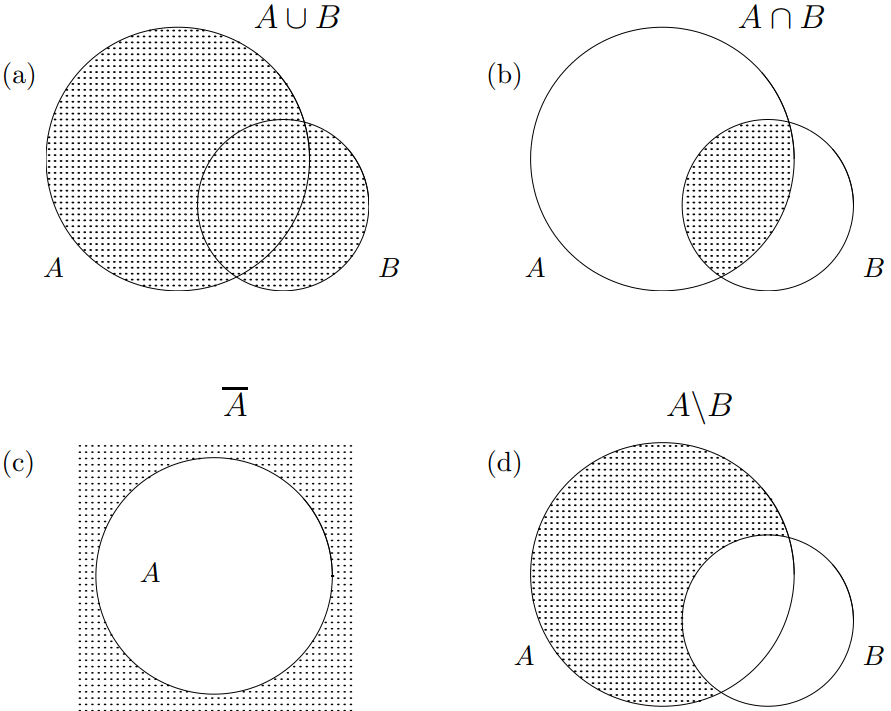
\includegraphics[width=.7\textwidth]{img/fig2.1.png}
    \caption{Venn diagrams for \textit{union}, \textit{intersection}, \textit{complement}, and \textit{difference} of events.}
\end{figure}

\begin{definition}{}
Events $A$ and $B$ are \textbf{disjoint} if their \textit{intersection is empty},
\begin{equation*}
    A \cap B = \emptyset
\end{equation*}
Events $A_1,\ A_2,\ A_3,\ ...$ are \textbf{mutually exclusive} or \textbf{pairwise disjoint} if any two of these events are disjoint, i.e.,
\begin{equation*}
    A_i \cap A_j = \emptyset \text{ for any } i \neq j
\end{equation*}
\end{definition}

If $E_1 \cap E_2 = \emptyset$, $E_1$ and $E_2$ are distinct, disjoint or mutually exclusive, events. One cannot observe both events at the same time, they do not have common outcome. 

On the other side, if $E_1 \cap E_2 \neq \emptyset$, $E_1$ and $E_2$ are not distinct events. One can observe \textit{both events at the same time}.

\begin{definition}{}
Events $A,\ B,\ C,\ ...$ are \textbf{exhaustive} if their union equals the whole sample space, i.e.,
\begin{equation*}
    A \cup B \cup C \cup \cdots = \Omega
\end{equation*}
\end{definition}

\begin{itemize}
    \item \textbf{Mutually exclusive} events will \textit{never occur at the same time}. Occurrence of any one of them eliminates the possibility for all the others to occur.
    \item \textbf{Exhaustive events} \textit{cover the entire $\Omega$}, so that “\textit{there is nothing left}.” In other words, among any collection of exhaustive events, at least one occurs for sure. Also, \textit{they do not have to be disjoint or single outcome events. Only union giving sample space enough for being exhaustive events.}
\end{itemize}

It is often easier to compute probability of an intersection than probability of a union. Taking complements converts unions into intersections.
\begin{align*}
    \overline{E_1 \cup \cdots \cup E_n} &= \overline{E_1} \cap \cdots \cap \overline{E_n}\\
    \overline{E_1 \cap \cdots \cap E_n} &= \overline{E_1} \cup \cdots \cup \overline{E_n}\\
\end{align*}
\begin{proof}
Since the union $E_1 \cup \cdots \cup E_n$ represents the event “\textit{at least one event occurs},” its complement has the form
\begin{align*}
    \overline{E_1 \cup \cdots \cup E_n} &= \text{\{none of them occurs\}}\\
    &= \text{\{$E_1$ does not occur $\cap \cdots \cap E_n$ does not occur\}}\\
    &= \overline{E_1} \cap \cdots \cap \overline{E_n}
\end{align*}
The other equality can be proved by using the same way.
\end{proof}

Rephrasing, a complement to “\textit{nothing}” is “\textit{something},” and “\textit{not everything}” means “\textit{at least one is missing}”


\section{Rules of Probability}

Mathematically, probability is introduced through several axioms.

\subsection{Axioms of Probability}

\textit{Not included.}

\subsection{Computing Probabilities of Events}

\subsubsection{Extreme Cases}

A sample space $\Omega$ consists of all possible outcomes, therefore, it occurs for sure. On the contrary, an empty event $\emptyset$ never occurs. So,
\begin{align*}
    &\textbf{\textit{P}}\{\Omega\} = 1 &\text{ and }& &\textbf{\textit{P}}\{\emptyset\} = 0
\end{align*}

\subsubsection{Union}

Consider an event that consists of some finite or countable collection of \textit{mutually exclusive outcomes},
\begin{equation*}
    E = \{\omega_1,\ \omega_2,\ \omega_3,\ ...\}
\end{equation*}
Summing probabilities of these outcomes, we obtain the probability of the entire event,
\begin{equation*}
    \textbf{\textit{P}}\{E\} = \sum_{\omega_k \in E} \textbf{\textit{P}}\{\omega_k\} = \textbf{\textit{P}}\{\omega_1\} + \textbf{\textit{P}}\{\omega_2\} + \textbf{\textit{P}}\{\omega_3\} + \cdots
\end{equation*}

It is crucial to notice that \textit{only mutually exclusive events} (those with empty intersections) satisfy the \textbf{sigma-additivity}. If events intersect, their probabilities cannot be simply added.

In the sum $\mathbf{P}\{A\} + \mathbf{P}\{B\}$, all the common outcomes are counted twice. Each outcome should be counted only once! To correct the formula, subtract probabilities of common outcomes, which is $\mathbf{P}\{A \cap B\}$.
\begin{align*}
    \textbf{\textit{P}}\{A \cup B\} &= \textbf{\textit{P}}\{A\} + \textbf{\textit{P}}\{B\} - \textbf{\textit{P}}\{A \cap B\}\\
    \textbf{\textit{P}}\{A \cup B\} &= \textbf{\textit{P}}\{A\} + \textbf{\textit{P}}\{B\} &\text{For mutually exclusive events}
\end{align*}

Generalization of this formula is not straightforward. For 3 events,
\begin{align*}
    \textbf{\textit{P}}\{A \cup B \cup C\} = \textbf{\textit{P}}\{A\} + \textbf{\textit{P}}\{B\} + \textbf{\textit{P}}\{C\} - \textbf{\textit{P}}\{A \cap B\} - \textbf{\textit{P}}\{A \cap C\} - \textbf{\textit{P}}\{B \cap C\} + \textbf{\textit{P}}\{A \cap B \cap C\}
\end{align*}

\subsubsection{Complement}

Recall that events $A$ and $\overline{A}$ are \textit{exhaustive}, hence $A \cup \overline{A} = \Omega$. Also, they are \textit{disjoint}, hence
\begin{equation*}
    \textbf{\textit{P}}\{A\} + \textbf{\textit{P}}\{\overline{A}\} = \textbf{\textit{P}}\{A \cup \overline{A}\} = \textbf{\textit{P}}\{\Omega\} = 1
\end{equation*}
Solving this for $\textbf{\textit{P}}\{A\}$, we obtain a rule that perfectly agrees with the common sense,
\begin{equation*}
    \textbf{\textit{P}}\{\overline{A}\} = 1 - \textbf{\textit{P}}\{A\}
\end{equation*}

\subsubsection{Intersection of Independent Events}

\begin{definition}
{}

Events $E_1,\ ..., E_n$ are \textbf{independent} if they occur \textit{independently of each other}, i.e., occurrence of one event does not affect the probabilities of other.
\end{definition}
The following basic formula can serve as the \textit{criterion of independence}.
\begin{equation*}
    \textbf{\textit{P}}\{E_1 \cap \cdots \cap E_n\} = \textbf{\textit{P}}\{E_1\} \times \cdots \times \textbf{\textit{P}}\{E_n\}
\end{equation*}

\subsection{Applications in Reliability}

Formulas of the previous section are widely used in \textit{reliability}, when one computes the probability for a system of several components to be functional.

\begin{example}{}
There is a 1\% probability for a hard drive to crash. Therefore, it has two backups, each having a 2\% probability to crash, and all three components are independent of each other. The stored information is lost only in an unfortunate situation when all three devices crash. What is the probability that the information is saved?

\textbf{Solution}:
Organize the data. Denote the events, say,
\begin{equation*}
    H = \{\text{hard drive crashes}\},\ \ 
    B_1 = \text{\{first backup crashes\}},\ \ B_2 = \text{\{second backup crashes\}}
\end{equation*}
It is given that $H,\ B_1$, and $B_2$ are independent,
\begin{equation*}
    \textbf{\textit{P}}\{H\} = 0.01,\ \ \textbf{\textit{P}}\{B_1\} = \textbf{\textit{P}}\{B_2\} = 0.02
\end{equation*}
Applying rules for the complement and for the intersection of independent events,
\begin{align*}
    \textbf{\textit{P}}\{\text{saved}\} &= 1 - \textbf{\textit{P}}\{\text{lost}\} = 1 - \textbf{\textit{P}}\{H \cap B_1 \cap B_2\}\\
    &= 1 - \textbf{\textit{P}}\{H\} \times \textbf{\textit{P}}\{B_1\} \times \textbf{\textit{P}}\{B_2\}\\
    &= 1 - (0.01)(0.02)(0.02) = 0.999996
\end{align*}
\end{example}

When the system’s components are connected in \textit{parallel}, it is sufficient for at least one component to work in order for the whole system to function. Reliability of such a system is computed as in example above. Backups can always be considered as devices connected in parallel.

At the other end, consider a system whose components are connected in \textit{sequel}. Failure of one component inevitably causes the whole system to fail. Such a system is more “vulnerable.” In order to function with a high probability, it needs each component to be reliable, as in the next example.

\begin{example}{}
Suppose that a shuttle’s launch depends on three key devices that operate independently of each other and malfunction with probabilities 0.01, 0.02, and 0.02, respectively. If any of the key devices malfunctions, the launch will be postponed. Compute the probability for the shuttle to be launched on time, according to its schedule.

\textbf{Solution:}
In this case,
\begin{align*}
    \textbf{\textit{P}}\{\text{on time}\} &= \textbf{\textit{P}}\{\text{all devices function}\}\\
    &= \textbf{\textit{P}}\{\overline{H} \cap \overline{B_1} \cap \overline{B_2}\} &\text{(independence)}\\
    &= \textbf{\textit{P}}\{\overline{H}\} \textbf{\textit{P}}\{\overline{B_1}\} \textbf{\textit{P}}\{\overline{B_2}\} &\text{(complement rule)}\\
    &= (1 - 0.01)(1 - 0.02)(1 - 0.02)\\
    &= 0.9508
\end{align*}
\end{example}


\section{Combinatorics}

\subsection{Equally Likely Outcomes}

A simple situation for computing probabilities is the case of \textit{equally likely outcomes}. That is, when the sample space $\Omega$ consists of $n$ possible outcomes, $\omega_1,\ ...,\ \omega_n$, each having the same probability. Since
\begin{equation*}
    \sum_{1}^{n} \textbf{\textit{P}}\{\omega_k\} = \textbf{\textit{P}}\{\Omega\} = 1
\end{equation*}
we have in this case $\textbf{\textit{P}}\{\omega_k\} = 1/n$ for all $k$. Further, a probability of any event $E$ consisting of $t$ outcomes, equals
\begin{equation*}
    \textbf{\textit{P}}\{E\} = \sum_{\omega_k \in E} \left( \frac{1}{n} \right) = t \left( \frac{1}{n} \right) = \frac{\text{number of outcomes in $E$}}{\text{number of outcomes in $\Omega$}}
\end{equation*}

\subsection{Permutations and Combinations}

\begin{itemize}
    \item \textbf{Sampling with replacement:} You can choose an object \textit{more than once}. Any object can be selected with $1/n$ probability at \textit{any time}.
    \item \textbf{Sampling with replacement:} Sampled item is removed. Set of possibilities \textit{reduces by 1} after every selection.
    \item \textbf{Distinguishable Objects:} Sampling of exactly the same objects in a \textit{different order yields a different outcome}.
    \item \textbf{Indistinguishable Objects:} The \textit{order is not important}. Differently arranged orders does not yield a different outcome.
\end{itemize}

\subsubsection{Permutations with Replacement}

Possible selections of $k$ \textit{distinguishable} objects from a set of $n$ are called \textbf{\textit{permutations}}.
\begin{formula}{Permutations with replacement}
\begin{equation*}
    P_r(n,k) = \overbrace{n \cdot n \cdot ... \cdot n}^{\text{k terms}} = n^k
\end{equation*}
\end{formula}

\subsubsection{Permutations without Replacement}

During selection, the number of possible selections reduces by 1 each time an object is sampled.
\begin{formula}{Permutations without replacement}
\begin{equation*}
    P(n,k) = \overbrace{n(n-1)(n-2) \cdot ... \cdot (n - k + 1)}^{\text{k terms}} = \frac{n!}{(n - k)!}
\end{equation*}
\end{formula}

\subsubsection{Combinations without Replacement}

Possible selections of $k$ \textit{indistinguishable} objects from a set of $n$ are called \textbf{combinations}. \textit{The only difference from $P(n,\ k)$ is \textbf{disregarding the order}}

\begin{formula}{Combinations without replacement}
\begin{equation*}
    C(n,k) = \binom{n}{k} = \frac{P(n,k)}{P(k,k)} = \frac{n!}{k! (n - k)!}
\end{equation*}
\end{formula}

\subsubsection{Computational Shortcuts}

\begin{align*}
    C(n,k) &= \binom{n}{k} = \frac{n \cdot (n-1) \cdot ... \cdot (n-k+1)}{k \cdot (k-1) \cdot ... \cdot 1}\\
    C(n,k) &= C(n, n-k) \text{   for any $k$ and $n$}\\
    C(n,0) &= 1\\
    C(n,1) &= n
\end{align*}

\subsubsection{Combinations with Replacement}

\begin{formula}{Combinations with replacement}
\begin{equation*}
    C_r(n,k) = \binom{k + n - 1}{k} = \frac{(k + n - 1)!}{k! (n - 1)!}
\end{equation*}
\end{formula}

\begin{formula}{\textit{NOTATION}}
\begin{align*}
    P_r(n, k) &= \text{number of permutations with replacement}\\
    P(n, k) &= \text{number of permutations without replacement}\\
    C_r(n, k) &= \text{number of combinations with replacement}\\
    C(n, k) &= \text{number of combinations without replacement}\\
    \binom{n}{k} &= \text{number of combinations without replacement}
\end{align*}
\end{formula}


\section{Conditional Probability and Independence}

\subsection{Conditional Probability}

\begin{definition}
\textbf{Conditional probability} of event $A$ given event $B$ is the probability that $A$ occurs when $B$ is known to occur.
\end{definition}

\textbf{\textit{NOTATION}}
\begin{equation*}
    \textbf{\textit{P}}\{A\ |\ B\} = \text{conditional probability of \textit{A} given \textit{B}}
\end{equation*}

\textit{Conditional probability basically is ``What is the probability of observing event $A$ given that event $B$ is observed?"}

How does one compute the conditional probability? First, consider the case of equally likely outcomes. In view of the new information, occurrence of the condition \textit{B}, only the outcomes contained in \textit{B} still have a non-zero chance to occur. Counting only such outcomes, the unconditional probability of \textit{A},
\begin{equation*}
    \textbf{\textit{P}}\{A\} = \frac{\text{number of outcomes in \textit{A}}}{\text{number of outcomes in $\Omega$}}
\end{equation*}
is now replaced by the conditional probability of \textit{A} given \textit{B},
\begin{equation*}
    \textbf{\textit{P}}\{A\ |\ B\} = \frac{\text{number of outcomes in $A \cap B$}}{\text{number of outcomes in $B$}} = \frac{\textbf{\textit{P}}\{A \cap B\}}{\textbf{\textit{P}}\{B\}}
\end{equation*}
This appears to be the general formula

\begin{formula}{Conditional Probability}
\begin{align*}
    \textbf{\textit{P}}\{A\ |\ B\} = \frac{\textbf{\textit{P}}\{A \cap B\}}{\textbf{\textit{P}}\{B\}}\\
    \textbf{\textit{P}}\{B\ |\ A\} = \frac{\textbf{\textit{P}}\{A \cap B\}}{\textbf{\textit{P}}\{A\}}
\end{align*}
\end{formula}

Rewriting in a different way, we obtain the general formula for the probability of intersection.

\begin{formula}{Intersection, general case}
\begin{align*}
    \textbf{\textit{P}}\{A \cap B\} = \textbf{\textit{P}}\{B\} \textbf{\textit{P}}\{A\ |\ B\}\\
    \textbf{\textit{P}}\{A \cap B\} = \textbf{\textit{P}}\{A\} \textbf{\textit{P}}\{B\ |\ A\}
\end{align*}
\end{formula}

\subsection{Independence}

\begin{definition}{}
Events $A$ and $B$ are \textbf{independent} if occurrence of $B$ does not affect the probability of $A$, i.e.,
\begin{align*}
    \textbf{\textit{P}}\{A\ |\ B\} = \textbf{\textit{P}}\{A\}\\
    \textbf{\textit{P}}\{B\ |\ A\} = \textbf{\textit{P}}\{B\}
\end{align*}
\end{definition}

\textit{So, if $\textbf{\textit{P}}\{A\ |\ B\} = \textbf{\textit{P}}\{A\}$ and $\textbf{\textit{P}}\{B\ |\ A\} = \textbf{\textit{P}}\{B\}$, it shows that $A$ and $B$ are \textbf{independent event}, the probability of observing $A\ |\ B$ is not affected by observing other event!}

According to this definition, \textit{conditional} probability equals \textit{unconditional} probability in case of independent events. Substituting this into formula of the probability of intersection:
\begin{equation*}
    \textbf{\textit{P}}\{A \cap B\} = \textbf{\textit{P}}\{A\} \textbf{\textit{P}}\{B\}
\end{equation*}

\textbf{Note:} If the equation $\textbf{\textit{P}}\{A\ |\ B\} = \textbf{\textit{P}}\{A\}$ does not hold, the events are not independent.

\begin{example}{}

Ninety percent of flights depart on time. Eighty percent of flights arrive
on time. Seventy-five percent of flights depart on time and arrive on time.
\begin{itemize}
    \item (a) You are meeting a flight that departed on time. What is the probability that it will arrive on time?
    \item (b) You have met a flight, and it arrived on time. What is the probability that it departed on time?
    \item (c) Are the events, departing on time and arriving on time, independent?
\end{itemize}

\textbf{Solution:} 
Denote the events,

\textit{A} = \{arriving on time\},  

\textit{D} = \{departing on time\}

We have:
\begin{align*}
    &\textbf{\textit{P}}\{A\} = 0.8 &\textbf{\textit{P}}\{D\} = 0.9& &\textbf{\textit{P}}\{A \cap D\} = 0.75
\end{align*}
\begin{itemize}
    \item (a) $\textbf{\textit{P}}\{A\ |\ D\} = \dfrac{\textbf{\textit{P}}\{A \cap D\}}{\textbf{\textit{P}}\{D\}} = \dfrac{0.75}{0.9} = 0.8333$
    \item (b) $\textbf{\textit{P}}\{D\ |\ A\} = \dfrac{\textbf{\textit{P}}\{A \cap D\}}{\textbf{\textit{P}}\{A\}} =\dfrac{0.75}{0.8} = 0.9375$
    \item (c) Events are not independent because
        \begin{align*}
            &\textbf{\textit{P}}\{A\ |\ D\} \neq \textbf{\textit{P}}\{A\} &\textbf{\textit{P}}\{D\ |\ A\} \neq \textbf{\textit{P}}\{D\}& &\textbf{\textit{P}}\{A \cap D\} \neq \textbf{\textit{P}}\{A\} \textbf{\textit{P}}\{D\}
        \end{align*}
\end{itemize}
Actually, any one of these inequalities is sufficient to prove that \textit{A} and \textit{D} are dependent. Further, we see that $\textbf{\textit{P}}\{A\ |\ D\} > \textbf{\textit{P}}\{A\}$ and $\textbf{\textit{P}}\{D\ |\ A\} > \textbf{\textit{P}}\{D\}$. In other words, departing on time increases the probability of arriving on time, and vice versa. This perfectly agrees with our intuition.
\end{example}

The following page belongs to \textbf{\textit{Berfinnur Oktay}}.

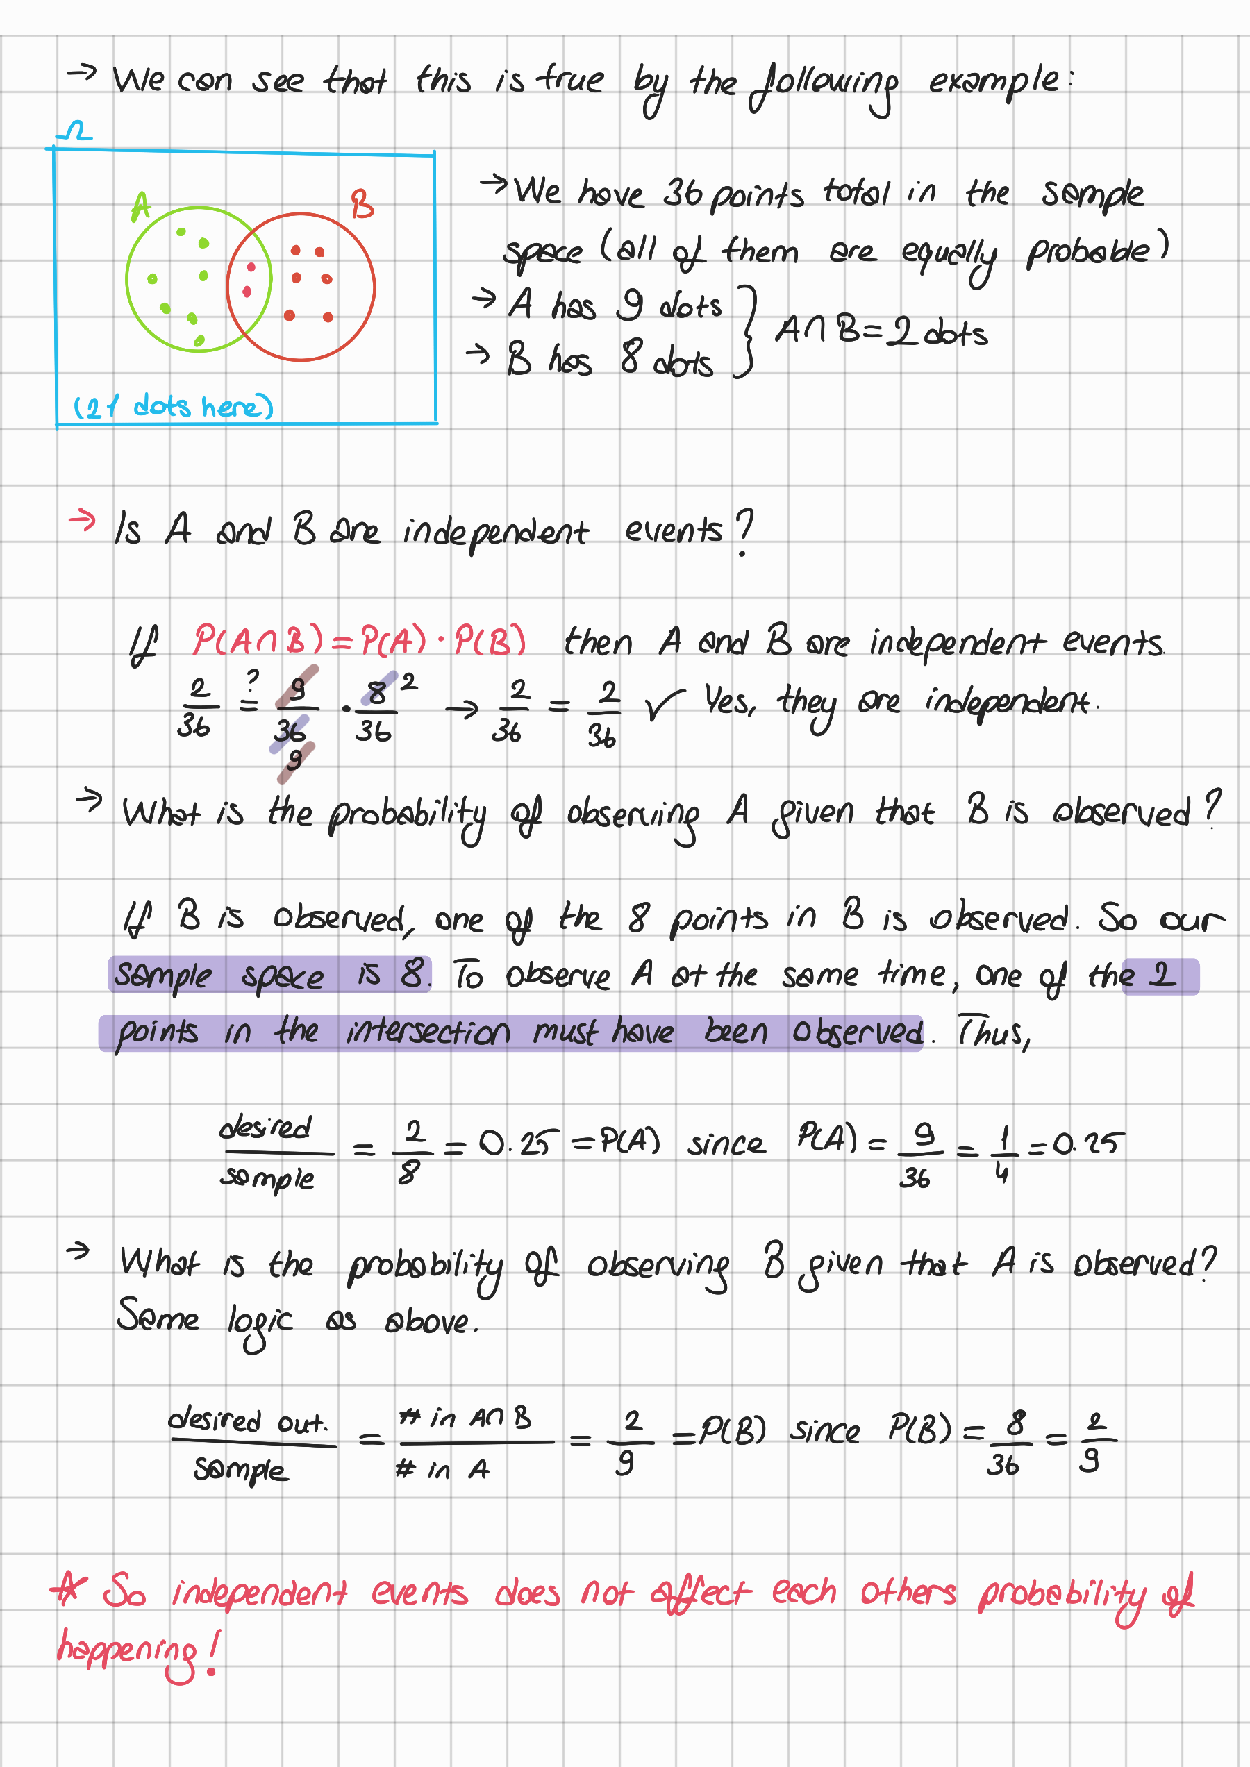
\includepdf[pages=-]{berf-notes-page-7.pdf}

\subsection{Bayes Rule}

Two conditional probabilities, $\textbf{\textit{P}}\{A\ |\ B\}$ and $\textbf{\textit{P}}\{B\ |\ A\}$, are not the same, in general.

\begin{example}{: Reliability of a test}
There exists a test for a certain viral infection (including a virus attack on a computer network). It is 95\% reliable for infected patients and 99\% reliable for the healthy ones. That is, if a patient has the virus (event $V$), the test shows that (event $S$) with probability $\textbf{\textit{P}}\{S\ |\ V\} = 0.95$, and if the patient does not have the virus, the test shows that with probability $\textbf{\textit{P}}\{\overline{S}\ |\ \overline{V}\} = 0.99$

Consider a patient whose test result is positive (i.e., the test shows that the patient has the virus). Knowing that sometimes the test is wrong, naturally, the patient is eager to know the probability that he or she indeed has the virus. However, this conditional probability, $\textbf{\textit{P}}\{V\ |\ S\}$, is not stated among the given characteristics of this test.
\end{example}

\noindent Notice that $A \cap B = B \cap A$. Therefore, $\prob{B} \prob{A\ |\ B} = \prob{A} \prob{B\ |\ A}$, by using the general case intersection formula,. Solve for $\prob{B\ |\ A}$ to obtain

\begin{formula}{Bayes Rule}
\begin{align*}
    \textbf{\textit{P}}\{B\ |\ A\} &= \frac{\textbf{\textit{P}}\{A\ |\ B\} \textbf{\textit{P}}\{B\}}{\textbf{\textit{P}}\{A\}}\\&\\
    \textbf{\textit{P}}\{A\ |\ B\} &= \frac{\textbf{\textit{P}}\{B\ |\ A\} \textbf{\textit{P}}\{A\}}{\textbf{\textit{P}}\{B\}}
\end{align*}
\end{formula}

\begin{example}{}
On a midterm exam, students $X$, $Y$, and $Z$ forgot to sign their papers. Professor knows that they can write a good exam with probabilities 0.8, 0.7, and 0.5, respectively. After the grading, he notices that two unsigned exams are good and one is bad. Given this information, and assuming that students worked independently of each other, what is the probability that the bad exam belongs to student $Z$?

\textbf{Solution:}
Denote good and bad exams by $G$ and $B$. Also, let $GGB$ denote two good and one bad exams, $XG$ denote the event “student $X$ wrote a good exam,” etc. We need to find $\textbf{\textit{P}}\{ZB\ |\ GGB\}$ given that $\textbf{\textit{P}}\{G\ |\ X\} = 0.8$, $\textbf{\textit{P}}\{G\ |\ Y\} = 0.7$, and $\textbf{\textit{P}}\{G\ |\ Z\} = 0.5$.

By the \textit{Bayes Rule},
\begin{equation*}
    \textbf{\textit{P}}\{ZB\ |\ GGB\} = \frac{\textbf{\textit{P}}\{GGB\ |\ ZB\} \textbf{\textit{P}}\{ZB\}}{\textbf{\textit{P}}\{GGB\}}
\end{equation*}
Given $ZB$, event $GGB$ occurs only when both $X$ and $Y$ write good exams. Thus,
$\textbf{\textit{P}}\{GGB\ |\ ZB\} = (0.8)(0.7)$.

Event $GGB$ consists of three outcomes depending on the student who wrote the bad exam. Adding their probabilities, we get
\begin{align*}
    \textbf{\textit{P}}\{GGB\} &= \textbf{\textit{P}}\{XG \cap YG \cap ZB\} + \textbf{\textit{P}}\{XG \cap YB \cap ZG\} + \textbf{\textit{P}}\{XB \cap YG \cap ZG\}\\
    &= (0.8)(0.7)(0.5) + (0.8)(0.3)(0.5) + (0.2)(0.7)(0.5) = 0.47 
\end{align*}
Then
\begin{equation*}
    \textbf{\textit{P}}\{ZB\ |\ GGB\} = \frac{(0.8)(0.7)(0.5)}{0.47} = 0.5957
\end{equation*}
\end{example}

Sometimes, it can be hard to determine the denominator in the \textit{Bayes Rule}. In the Bayes Rule, the denominator is often computed by the \textbf{Law of Total Probability}.

\subsection{Law of Total Probability}

This law relates the \textit{unconditional probability of an event $A$} with its \textit{conditional probabilities}. It is used every time when it is easier to compute conditional probabilities of $A$ given additional information.

\begin{figure}[ht!]
    \centering
    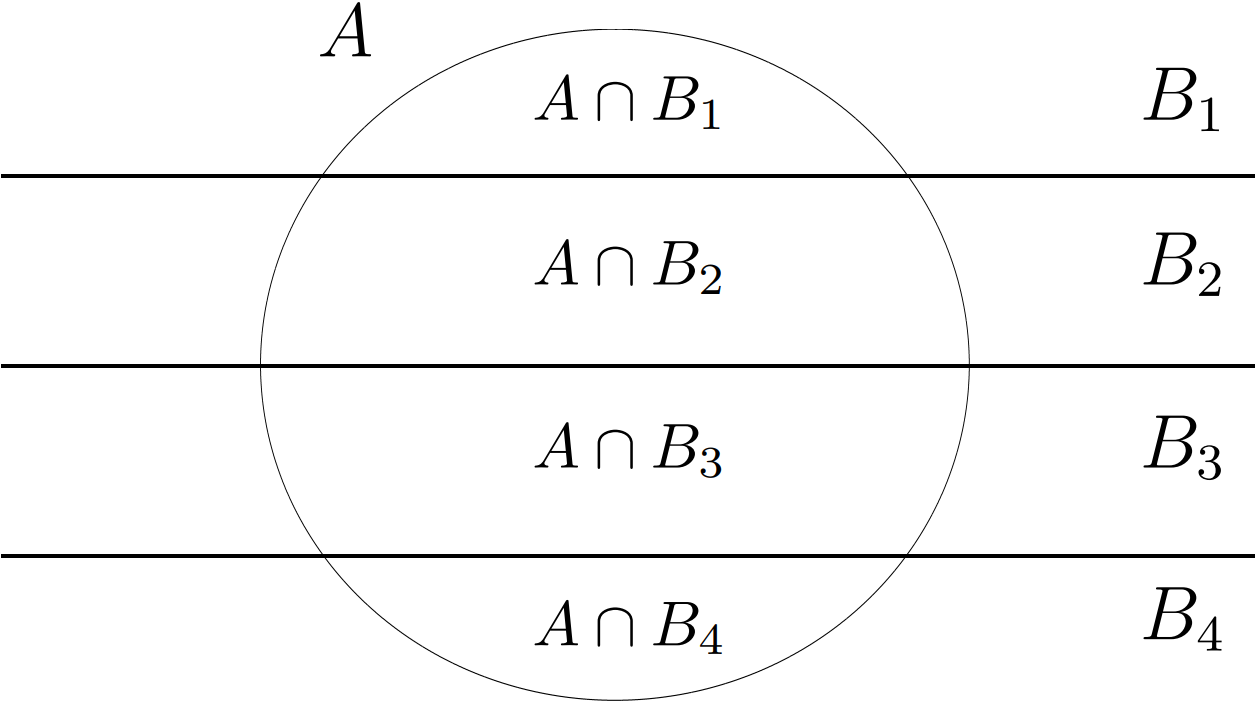
\includegraphics[width=.6\textwidth]{img/fig2.6.png}
    \caption{Partition of the sample space $\Omega$ and the event $A$}
\end{figure}

Consider some partition of the sample space $\Omega$ with \textit{mutually exclusive} and \textit{exhaustive} events $B_1,\ ...,\ B_k$. It means that
\begin{equation*}
    B_i \cap B_j = \emptyset \text{ for any } i \neq j \text{ and } B_1 \cup \cdots \cup B_k = \Omega
\end{equation*}
These events also partition the event $A$
\begin{equation*}
    A = (A \cap B_1) \cup \cdots \cup (A \cap B_k)
\end{equation*}
and this is also a union of mutually exclusive events. Hence,
\begin{equation*}
    \textbf{\textit{P}}\{A\} = \sum_{j = 1}^{k} \textbf{\textit{P}}\{A \cap B_j\}
\end{equation*}
and we arrive to the following rule.

\begin{formula}{Law of Total Probability}
\begin{equation*}
    \textbf{\textit{P}}\{A\} = \sum_{j = 1}^{k} \textbf{\textit{P}}\{A\ |\ B_j\} \textbf{\textit{P}}\{B_j\}
\end{equation*}
In case of two events ($k = 2$),
\begin{equation*}
    \textbf{\textit{P}}\{A\} = \textbf{\textit{P}}\{A\ |\ B\} \textbf{\textit{P}}\{B\} + \textbf{\textit{P}}\{A\ |\ \overline{B}\} \textbf{\textit{P}}\{\overline{B}\}
\end{equation*}
\end{formula}
Together with the Bayes Rule, it makes the following popular formula
\begin{formula}{Bayes Rule for two events}
\begin{align*}
    \textbf{\textit{P}}\{B\ |\ A\} &= \frac{\textbf{\textit{P}}\{A\ |\ B\} \textbf{\textit{P}}\{B\}}{\textbf{\textit{P}}\{A\ |\ B\} \textbf{\textit{P}}\{B\} + \textbf{\textit{P}}\{A\ |\ \overline{B}\} \textbf{\textit{P}}\{\overline{B}\}}\\&\\
    \textbf{\textit{P}}\{A\ |\ B\} &= \frac{\textbf{\textit{P}}\{B\ |\ A\} \textbf{\textit{P}}\{A\}}{\textbf{\textit{P}}\{B\ |\ A\} \textbf{\textit{P}}\{A\} + \textbf{\textit{P}}\{B\ |\ \overline{A}\} \textbf{\textit{P}}\{\overline{A}\}}
\end{align*}
\end{formula}

\begin{example}{: Reliability of a test, continued}
Suppose that 4\% of all the patients are infected with the virus, $\textbf{\textit{P}}\{V\} = 0.04$. Recall that $\textbf{\textit{P}}\{S\ |\ V\} = 0.95$ and $\textbf{\textit{P}}\{\overline{S}\ |\ \overline{V}\} = 0.99$. If the test shows positive results, the (conditional) probability that a patient has the virus equals
\begin{align*}
    \textbf{\textit{P}}\{V\ |\ S\} 
    &= \frac{\textbf{\textit{P}}\{S\ |\ V\}\textbf{\textit{P}}\{V\}}{\textbf{\textit{P}}\{S\ |\ V\} \textbf{\textit{P}}\{V\} + \textbf{\textit{P}}\{S\ |\ \overline{V}\} \textbf{\textit{P}}\{\overline{V}\}}\\
    &= \frac{(0.95)(0.04)}{(0.95)(0.04) + (1 - 0.99)(1 - 0.04))} = 0.7983
\end{align*}
\end{example}

\textit{Check the example 2.35 from book.}

\end{document}
